\documentclass{beamer}
\usetheme{Antibes}
\usecolortheme{orchid}
\usepackage{amsmath}
\usepackage[utf8]{inputenc}
\usepackage{tikz}
\usepackage{graphicx}
\graphicspath{ {./} }

\def\insertauthorindicator{Who?}% Default is "Who?"
\def\insertinstituteindicator{From?}% Default is "From?"
\def\insertdateindicator{When?}% Default is "When?"

\title{Neural networks}
\subtitle{Architectures and training tips}

\author{Sebastian Bj{\"o}rkqvist}
\institute{IPRally Technologies}

\date[09.01.2019]{09.01.2019}

\newcommand{\kur}{\protect\textit}
\newcommand{\bol}{\protect\textbf}
\newcommand\pro{\item[$+$]}
\newcommand\con{\item[$-$]}

\def\layersep{2.2cm}
\begin{document}

\frame{\titlepage}
  \begin{frame}
    \frametitle{What is a neural network?}  
    
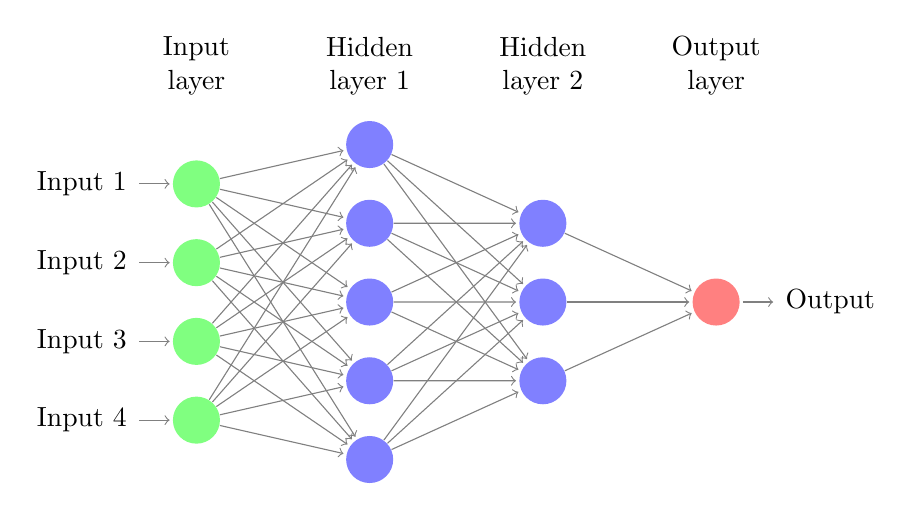
\begin{tikzpicture}[shorten >=1pt,->,draw=black!50, node distance=\layersep]
    \tikzstyle{every pin edge}=[<-,shorten <=1pt]
    \tikzstyle{neuron}=[circle,fill=black!25,minimum size=17pt,inner sep=0pt]
    \tikzstyle{input neuron}=[neuron, fill=green!50];
    \tikzstyle{output neuron}=[neuron, fill=red!50];
    \tikzstyle{hidden neuron}=[neuron, fill=blue!50];    
    \tikzstyle{hidden neuron 2}=[neuron, fill=blue!50];
    \tikzstyle{annot} = [text width=4em, text centered]

    % Draw the input layer nodes
    \foreach \name / \y in {1,...,4}
    % This is the same as writing \foreach \name / \y in {1/1,2/2,3/3,4/4}
        \node[input neuron, pin=left:Input \y] (I-\name) at (0,-\y) {};

    % Draw the hidden layer nodes
    \foreach \name / \y in {1,...,5}
        \path[yshift=0.5cm]
            node[hidden neuron] (H-\name) at (\layersep,-\y cm) {};

    % Draw the hidden layer nodes
    \foreach \name / \y in {1,...,3}
        \path[yshift=-0.5cm]
            node[hidden neuron 2] (F-\name) at (2*\layersep,-\y cm) {};

    % Draw the output layer node
    \node[output neuron,pin={[pin edge={->}]right:Output}, right of=F-2] (O) {};

    % Connect every node in the input layer with every node in the
    % hidden layer.
    \foreach \source in {1,...,4}
        \foreach \dest in {1,...,5}
            \path (I-\source) edge (H-\dest);
    \foreach \source in {1,...,5}
        \foreach \dest in {1,...,3}
            \path (H-\source) edge (F-\dest);

    % Connect every node in the hidden layer with the output layer
    \foreach \source in {1,...,3}
        \path (F-\source) edge (O);

    % Annotate the layers
    \node[annot,above of=H-1, node distance=1cm] (hl) {Hidden layer 1};
    \node[annot,right of=hl, node distance=\layersep] (fl) {Hidden layer 2};
    \node[annot,left of=hl] {Input layer};
    \node[annot,right of=fl] {Output layer};
\end{tikzpicture}

  \tiny Modified from \url{http://www.texample.net/tikz/examples/neural-network/}
  \end{frame}

  \begin{frame}
    \frametitle{What is a neural network?}  
    At each hidden layer node $i$ the output value is calculated by 
	\begin{align*}
    o_{i} = \sigma(\sum{w_{ki}o_{ki-1}} + b_{i}). 
    \end{align*}
    \onslide<2->{The function $\sigma$ is called the activation function. It must be non-linear to allow the network to learn non-linear dependencies.}
  \end{frame} 
  \begin{frame}
    \frametitle{Why neural networks?}  
    
   	\begin{itemize}
		\item Can approximate any function \cite{hornik}
		\onslide<2->{\item May learn to respond to unexpected patterns}
		\onslide<3->{\item Useful especially when the amount of data is large}
		\onslide<4->{\item Less need for feature engineering compared to traditional ML methods}
	\end{itemize}
  \end{frame}
  
  \begin{frame}
    \frametitle{Recurrent neural network (RNN)}  
    
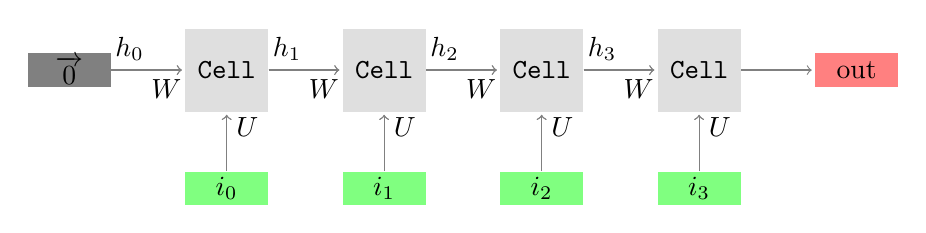
\begin{tikzpicture}[shorten >=1pt,->,draw=black!50, node distance=\layersep]
    \tikzstyle{every pin edge}=[<-,shorten <=1pt]
    \tikzstyle{vector}=[rectangle,fill=black!25,minimum width =30pt, minimum height=12pt,inner sep=0pt]    
    \tikzstyle{cell}=[rectangle,fill=gray!25,minimum width =30pt, minimum height=30pt,inner sep=0pt, font=\ttfamily]
    \tikzstyle{input vector}=[vector, fill=green!50];
    \tikzstyle{hidden vector}=[vector, fill=blue!50];
    \tikzstyle{output vector}=[vector, fill=red!50];
    \tikzstyle{zero vector}=[vector, fill=black!50];        
    \tikzstyle{annot} = [text width=4em, text centered]

        \node[zero vector] (H-0) at (0,-1) {$\overrightarrow{0}$};
        \foreach \name / \y in {1,...,4}
        	\node[cell] (C-\y) at (2*\y,-1) {Cell};
        \foreach \name / \y in {0,...,3}
        	\node[input vector] (I-\y) at (2*\y + 2,-2.5) {$i_{\y}$};
        \node[output vector] (O) at (10,-1) {out};

	\path (H-0) edge node[near start, above] {$h_{0}$} (C-1);
	\path (H-0) edge node[near end, below] {$\bold{W}$} (C-1);
	
    \foreach \y [count=\i] in {2,...,4}
    	\path (C-\i) edge node[near start, above] {$h_{\i}$}(C-\y);
    \foreach \y [count=\i] in {2,...,4}
    	\path (C-\i) edge node[near end, below] {$\bold{W}$}(C-\y);

	\path (C-4) edge (O);
	
	\foreach \y [count=\i] in {0,...,3}
		\path (I-\y) edge (C-\i); 
	\foreach \y [count=\i] in {0,...,3}
		\path (I-\y) edge node[near end, right]{$\bold{U}$}(C-\i);   	


\end{tikzpicture}  
	
	Processes each element of the input sequence in order, and keeps information about the past elements in a hidden state vector.

  \end{frame}  
  
  \begin{frame}
    \frametitle{Recurrent neural network (RNN)}  
    
	At each timestep $t$ the new hidden state is calculated using the new input at this timestep and the existing hidden state. The most basic version is the following:
	
	\begin{align*}
    h_{t} = \sigma(Wh_{t-1} + Ui_{t} + b). 
    \end{align*}	
	
  \onslide<2->{Other RNN architectures (for instance LSTM or GRU) use more complicated ways of updating the hidden state to control the flow of information to and from the hidden state.}
  \end{frame}      
  
  \begin{frame}
    \frametitle{RNN pros and cons}  
    
   	\begin{itemize}
		\onslide<2->{\pro Accepts input of variable size, i.e. sequences (time series, sentences etc)}
		\onslide<3->{
		\begin{itemize}
				\item{Can even be used to process tree-structured inputs by using Tree-LSTMs \cite{tai}}
		\end{itemize}}			
		\onslide<4->{\pro May learn long-term dependencies}
		\onslide<5->{\con Training may be slow when sequence length is large}
		
	\end{itemize}
  \end{frame}    

  \begin{frame}
    \frametitle{RNN real life use case: Patent search}  
    
	At IPRally we work on automated patent searches. The basic idea is the following:
	
	\begin{enumerate}
		\onslide<2->{\item Patents are transformed to graphs by extracting the relevant information from the patent claims and specifications}
		\onslide<3->{\item The graphs are then embedded to vectors by using a Tree-LSTM model}
		\begin{itemize}
			\onslide<4->{\item {The model is trained by using millions of real-life positive and negative novelty citations from previous patent applications}}
			\onslide<5->{\item {Patents with a positive citation get vectors that are close to each other}}
		\end{itemize}
		\onslide<6->{\item A prior art search for a new patent can then be done by searching for the nearest neighbors of the vector created from the new invention}
	\end{enumerate}

  \end{frame}    

  \begin{frame}
    \frametitle{RNN real life use case: Patent search}  
  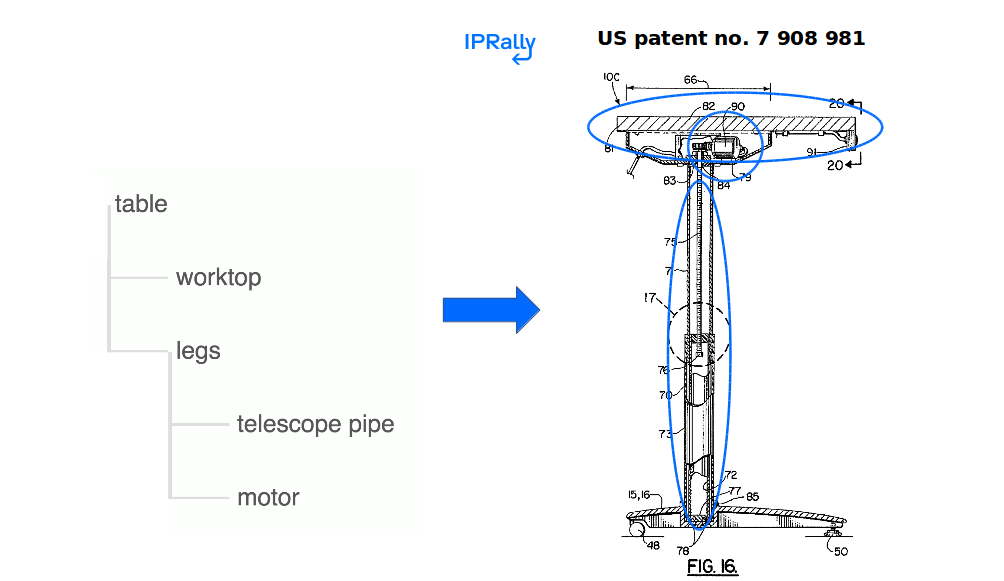
\includegraphics[scale=0.32]{patent_search_iprally_slide_20190106} 
  \end{frame}

  \begin{frame}
    \frametitle{Convolutional neural network (CNN)}  
    
	TODO: Picture here    

  Extracts features of two-dimensional input (usually an image) using convolutional and pooling layers.

  \end{frame}  
  
  \begin{frame}
    \frametitle{CNN pros and cons}  
    
   	\begin{itemize}
		\onslide<2->{\pro Works well with image data}
		\onslide<3->{\pro Training can be effectively parallelized}
		\onslide<4->{\pro Pre-existing models can be fine-tuned for specific tasks}
		\onslide<5->{\con Does not take into account position or orientation of the object}
	\end{itemize}
  \end{frame}    

  \begin{frame}
    \frametitle{Challenges when training neural networks}  
    
   	\begin{itemize}
		\onslide<2->{\item Finding the optimal neural network layout is often time-consuming}
		\onslide<3->{\item The model may be sensitive to changes in hyperparameters}
		\onslide<4->{\item A model may take several hours or even days to train}
		\onslide<4->{
		\begin{itemize}
				\item{This makes hyperparameter searches very expensive}
		\end{itemize}}		
		

	\end{itemize}
  \end{frame}  

  \begin{frame}
    \frametitle{Tips and tricks}  
    
   	\begin{itemize}
		\item Write unit tests for your model \cite{roberts}
		\begin{itemize}
      		\item{Check that each layer actually changes weights}
      		\item{Make sure that model converges on tiny data set}
    	\end{itemize}
		\onslide<2->{\item Stick to well-known architectures when starting out (e.g. LSTM/GRU for sequential data)}
		\onslide<3->{\item Start by using small batch size
		\begin{itemize}
      		\item{Usually makes model less sensitive to other hyperparameters}
      	\end{itemize}}
		\onslide<4->{\item Use normalization (batch, layer, group, weight...)
		\begin{itemize}
			\item Speeds up convergence significantly
      		\item{Start by trying batch normalization for CNN and feed-forward nets and layer normalization for RNN}}
    	\end{itemize}		
	\end{itemize}
  \end{frame}  

  \begin{frame}
    \frametitle{The curious case of the batch size}  
  
  \begin{itemize}
  	\item Training of neural nets can be sped up by increasing the batch size, since then the GPU/TPU can process more training examples in parallel
  	\item Unfortunately increasing the batch size may result in a worse model. In extreme cases the model might not learn anything at all! \cite{masters}
  	\item The basic rule is to increase the learning rate linearly when increasing the batch size (e.g. double learning rate when doubling batch size)
	\begin{itemize}
		\item Otherwise the magnitude of the weight updates decreases
    \end{itemize}
    \item This means that increasing the batch size trades computational efficiency for stale gradients.  	
  \end{itemize}

  \end{frame}  


%   
   \begin{frame}
   	\frametitle{References}
   	\begin{thebibliography}{Hornik, 1991}

  \bibitem[Nielsen, 2015]{nielsen} Nielsen, Michael A. {\em Neural Networks And Deep Learning}. Determination Press, 2015. \url{http://neuralnetworksanddeeplearning.com/}
  
  \bibitem[Hornik, 1991]{hornik} Hornik, Kurt. {\em Approximation Capabilities of Multilayer Feedforward Networks}. Neural Networks, 4(2), 251--257, 1991.
  
  \bibitem[Roberts, 2017]{roberts} Roberts, Chase. \em{How to unit test machine learning code.} Medium.com 2017. \url{https://medium.com/@keeper6928/how-to-unit-test-machine-learning-code-57cf6fd81765}.
  
  \bibitem[Tai et. al., 2015]{tai} Tai, Kai Sheng et al. \em{Improved Semantic Representations From Tree-Structured Long Short-Term Memory Networks.} ACL 2015. \url{https://arxiv.org/abs/1503.00075}
   
  \bibitem[Masters et. al., 2018]{masters} Masters, Dominic, Luschi, Carlo. \em{Revisiting Small Batch Training for Deep Neural Networks.} arXiv preprint 2018. \url{https://arxiv.org/abs/1804.07612}
   
	\end{thebibliography}   
   \end{frame}  

\end{document}
